%% Included in decks: slidemage-manual
%%

% SlideMage manual, chapter "Working in SlideMage": the side panels (the upper part of the
% workspace's right column). The strip is a crop of the Visibility panel
% (tools/manual/make_screenshots.py, shot panel-visibility).
\setSlideVersion{1-0-0}
\begin{standardframe}{Side panels}
	\small
	The upper part of the right column shows one panel about the focused slide; the arrow beside its name picks which.
	\par\smallskip
	\centering
	{\setlength{\fboxsep}{0pt}\fcolorbox{c_primary_gray}{white}{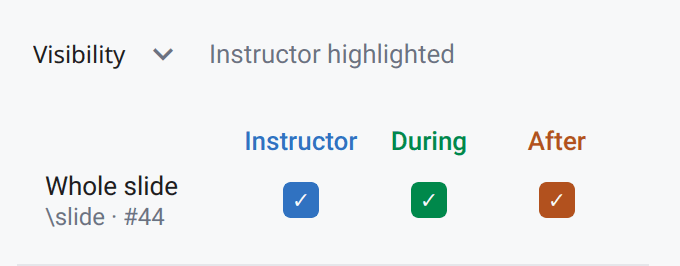
\includegraphics[width=\dimexpr0.3\linewidth-0.8pt\relax]{media/screenshot-slidemage-side-panel.png}}}
	\par\smallskip
	\raggedright
	\begin{columns}[T,onlytextwidth]
		\begin{column}{0.48\linewidth}
			\shrinklists{2}
			\begin{itemize}
				\item \emph{Used in decks}: the decks that call the slide, and which version they follow
				\item \emph{Slide versions}: freeze, open and restore versions
				\item \emph{Visibility}: the views (Instructor, During, After) the slide appears in
				\item \emph{Citations}: the references the slide cites, from \SMCode{Slidemaster.bib}
			\end{itemize}
		\end{column}
		\begin{column}{0.48\linewidth}
			\shrinklists{2}
			\begin{itemize}
				\item \emph{Language}: the slide's language and translations
				\item \emph{Image descriptions}: the slide's images and their texts
				\item \emph{Transcript entry}: an optional summary for the transcript
				\item \emph{Speaker notes}: the \SMCmd{note} text, instructor only
			\end{itemize}
		\end{column}
	\end{columns}
\end{standardframe}
